\documentclass[a4paper,11pt]{jsarticle}


% 文字
\usepackage{otf} % ギリシャ数字

% 数式
\usepackage{amsmath,amsfonts,amssymb}
\usepackage{bm}

% 表・画像共用
\usepackage{float} % 配置
% 画像
\usepackage[dvipdfmx]{graphicx} % 挿入
% 表や図のサイズ
\usepackage{graphicx}
% リスト
\usepackage{listings,jlisting} 
\renewcommand{\lstlistingname}{リスト}
\lstset{
  basicstyle={\ttfamily},
  identifierstyle={\small},
  commentstyle={\smallitshape},
  keywordstyle={\small\bfseries},
  stringstyle={\small\ttfamily},
  frame={tb},
  ndkeywordstyle={\small},
  breaklines=true,
  columns=[l]{fullflexible},
  numbers=left,
  xrightmargin=0zw,
  xleftmargin=3zw,
  numberstyle={\scriptsize},
  stepnumber=1,
  numbersep=1zw,
  lineskip=-0.5ex
}

% URL
\usepackage{url}


\begin{document}

\title{アナログ時計アプリの起動方法と操作方法}
\author{4年 電子情報工学科 川原隼平}
\date{}
\maketitle
  \section{起動方法}\label{sec:startup}
    \ref{sec:startup}章ではアナログ時計アプリの起動方法を説明する。
    以下に起動方法を示す。
    ただしMakefile と同じフォルダに j18411.exe というファイルがある場合は、
    基本的に手順3のみを行えばよい。

    \begin{enumerate}
      \item コマンドライン上で Makefile と同じフォルダに移動する。
      \item コマンドライン上で make と入力する。
      これを行うことでソースファイルがビルドされ、 Makefile と同じフォルダに j18411.exe という
      ファイルが生成される。
      \item コマンドライン上で ./j18411.exe と入力する。これを行うことでアナログ時計アプリが起動する。
    \end{enumerate}

  \section{操作方法}\label{sec:control}
    \ref{sec:control}章ではアナログ時計アプリの操作方法を説明する。
    \ref{sec:startup}章にしたがって起動した際に表示される画面を図\ref{fig:startup}に示す。
    また、操作方法を説明するために図\ref{fig:startup}に囲みをつけたものを図\ref{fig:startup-control}に示す

    \begin{figure}[H]
      \centering
      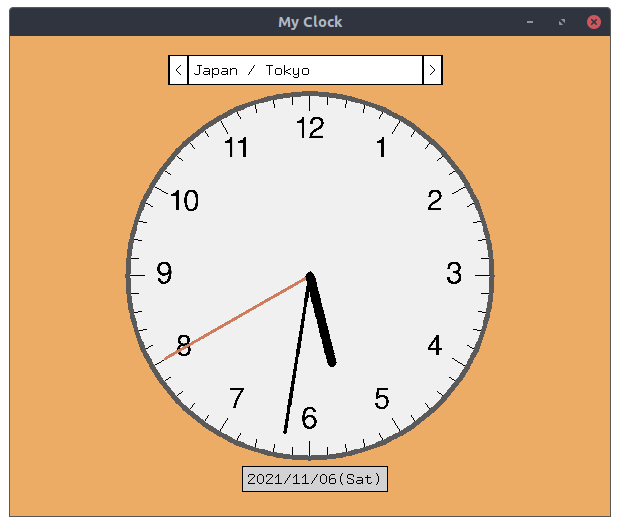
\includegraphics[scale=0.3]{./src/startup.png}
      \caption{起動後の画面}
      \label{fig:startup}
    \end{figure}

    \begin{figure}[H]
      \centering
      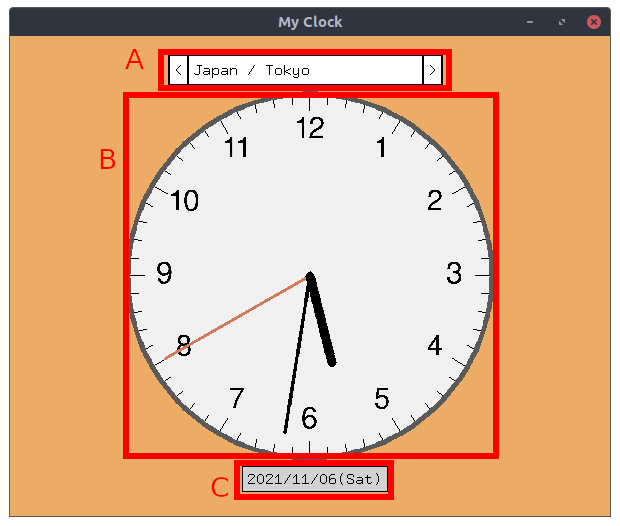
\includegraphics[scale=0.3]{./src/startup_control.png}
      \caption{操作方法を説明するために囲みをつけたもの}
      \label{fig:startup-control}
    \end{figure}

    図\ref{fig:startup-control}のように、画面起動時は囲みBに時計,囲みCに年月日と曜日が表示される。
    画面起動時に表示されている日時は東京の日時である。
    また、背景色は午前だと水色,午後だとオレンジ色になる。
    図\ref{fig:startup}や図\ref{fig:startup}は午後に写真を撮影したため背景色がオレンジ色になっている。

    囲みAはどの都市の日時を画面に表示するかを変更するためのボタンである。
    囲みAの中央のテキストボックスでは、現在どの都市の日時を表示しているかを表している。
    どの都市の日時を画面に表示するかは囲みAの左右のボタンを操作することで変更できる。
    以下に示す都市に対応している。ただしサマータイムは対応していない。

    \begin{itemize}
      \item 北京(中国)
      \item カイロ(エジプト)
      \item デリー(インド)
      \item ホノルル(アメリカ)
      \item ロンドン(イギリス)
      \item ニューヨーク(アメリカ)
      \item パリ(フランス)
      \item サンフランシスコ(アメリカ)
      \item 東京(日本)
    \end{itemize}
    

\end{document}

